\documentclass{article}
\usepackage[utf8]{inputenc}
\usepackage{hyperref}
\usepackage{listings}
\usepackage{wrapfig}
\usepackage{graphicx}
\usepackage{float} 
\usepackage{amsmath}
\usepackage{authblk}
\usepackage[spanish]{babel}
\usepackage[utf8]{inputenc}
\usepackage[backend=biber]{biblatex}
\bibliography{referencias}

\title{Prediccion de la facuturacion de la energia electrica en electro puno usando regresion lineal y python}
\author{Jose Angel Condori Ccapa, {\textit {angel.cc@upeu.edu.pe}}}

\begin{document}
\maketitle
\section{Resumen}

En este artículo, se presenta un estudio sobre la predicción de la facturación de la energía eléctrica en el departamento de Puno, utilizando técnicas de regresión lineal y programación en Python. La energía eléctrica es un recurso vital en la región de Puno, y es importante poder predecir la facturación para fines de planificación y gestión eficiente.
\\

En primer lugar, se aplicó la regresión lineal simple para modelar la relación entre el consumo de energía y la facturación. Se encontró una relación lineal positiva entre estas variables, lo que indica que a medida que aumenta el consumo, también lo hace la facturación. Se calcularon los coeficientes de la ecuación de regresión, incluyendo el intercepto y la pendiente.
\\

Posteriormente, se llevó a cabo una regresión lineal múltiple para incorporar una segunda variable independiente: el ubigeo de la persona. Se encontró que el consumo y el ubigeo son factores significativos en la predicción de la facturación. Se calcularon los coeficientes correspondientes a cada variable independiente en la ecuación de regresión.
\\

Se implementó el análisis utilizando Python y diversas bibliotecas, como numpy, pandas y matplotlib. Los datos fueron cargados, limpiados y procesados para su análisis. Se generaron gráficos de dispersión y se trazaron las líneas de regresión para visualizar la relación entre las variables.
\\

\textbf{palabras clase}: Ciencia de datos, Consumo de energia electrica, Regresion lineal simple y  Reresion lineal multiple

\section{Introduccion}
La predicción precisa de la facturación de la energía eléctrica es esencial para las empresas de distribución eléctrica, ya que les permite planificar y gestionar de manera eficiente la producción y distribución de energía, optimizar los recursos y mejorar la rentabilidad. En este contexto, el uso de técnicas de análisis de datos y modelado se ha vuelto fundamental para realizar pronósticos precisos y confiables.
\\

En este estudio, se propone la aplicación de la regresión lineal como una herramienta para predecir los niveles de facturación de la energía eléctrica en la empresa Electro Puno. La regresión lineal es un método estadístico que busca establecer una relación lineal entre una variable dependiente (la facturación eléctrica en este caso) y una o más variables independientes (como el consumo de energía, la temperatura, la estacionalidad, entre otros)
\\

El objetivo principal de este estudio es evaluar la eficacia de la regresión lineal en la predicción de la facturación de la energía eléctrica en Electro Puno, así como identificar las variables más influyentes en dicho proceso. Los resultados obtenidos en este análisis podrían proporcionar a Electro Puno información valiosa para la toma de decisiones relacionadas con políticas tarifarias, eficiencia energética y estrategias de demanda.
\section{Marco Teorico}
\subsection{Electro puno}
Electro Puno es una empresa estatal peruana que se dedica a la generación, transmisión y distribución de energía eléctrica en la región de Puno, ubicada en el sur del Perú. Es una de las empresas eléctricas del país y forma parte del Grupo Electro Perú, junto con otras empresas estatales del sector eléctrico.
\\

Electro Puno se encarga de operar y mantener las instalaciones eléctricas en su área de concesión, que abarca la región de Puno y parte de la región de Madre de Dios. Su objetivo principal es garantizar el suministro de energía eléctrica a los usuarios de la zona, tanto residenciales como comerciales e industriales.

\subsection{Regresion lineal simple}
La regresión lineal simple es un método estadístico utilizado para modelar la relación entre una variable dependiente (variable a predecir) y una única variable independiente (variable predictora). Se basa en la suposición de que existe una relación lineal entre las dos variables.
\\

En la regresión lineal simple, se busca encontrar la línea recta que mejor se ajusta a los puntos de datos en un gráfico de dispersión. Esta línea recta se conoce como "línea de regresión" y se representa mediante una ecuación de la forma:

\[
  y = \beta_0 + \beta_1x .   
\]

\begin{itemize}
  \item y = variable dependiente o variable a predecir
  \item \( \beta_0 \) = El intercepto 
  \item \( \beta_1 \) = La pendiente
  \item \( x \) = variable independiente
\end{itemize}


\subsection{Regresion lineal multiple}


La regresión lineal múltiple es una extensión de la regresión lineal simple que permite modelar la relación entre una variable dependiente y múltiples variables independientes. En lugar de utilizar una única variable predictora como en la regresión lineal simple, la regresión lineal múltiple utiliza varias variables independientes para predecir la variable dependiente.

\[ y = \beta_0 + \beta_1x_1 + \beta_2x_2 + \ldots + \beta_nx_n \]
\begin{itemize}
  \item y = variable dependiente o variable a predecir
  \item \( \beta_0 \) = El intercepto 
  \item \( \beta_1 ...... \beta_n \) = La pendiente
  \item \( x_1......x_n \) = variable independiente
\end{itemize}
\section{Metodologia}
los datos mostrados en este estudio estan en el siguiente enlace: \href{https://www.datosabiertos.gob.pe/dataset/consumo-de-energ%C3%ADa-el%C3%A9ctrica-de-los-clientes-de-electro-puno-saa}{Electro Puno}

Diccionario de datos

\begin{figure}[H]
  \centering
  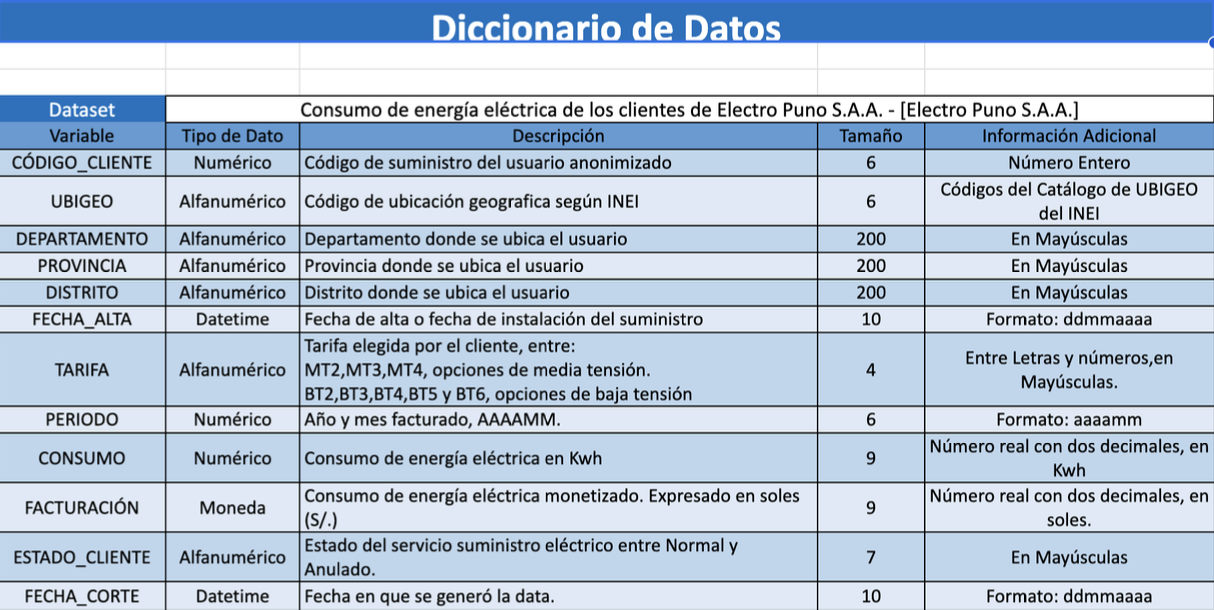
\includegraphics[width=1\textwidth]{./img/datos.png}
  \caption{Diccionario de datos}
  \label{Diccionario de datos}
\end{figure}

Tabla de datos
\begin{figure}[H]
  \centering
  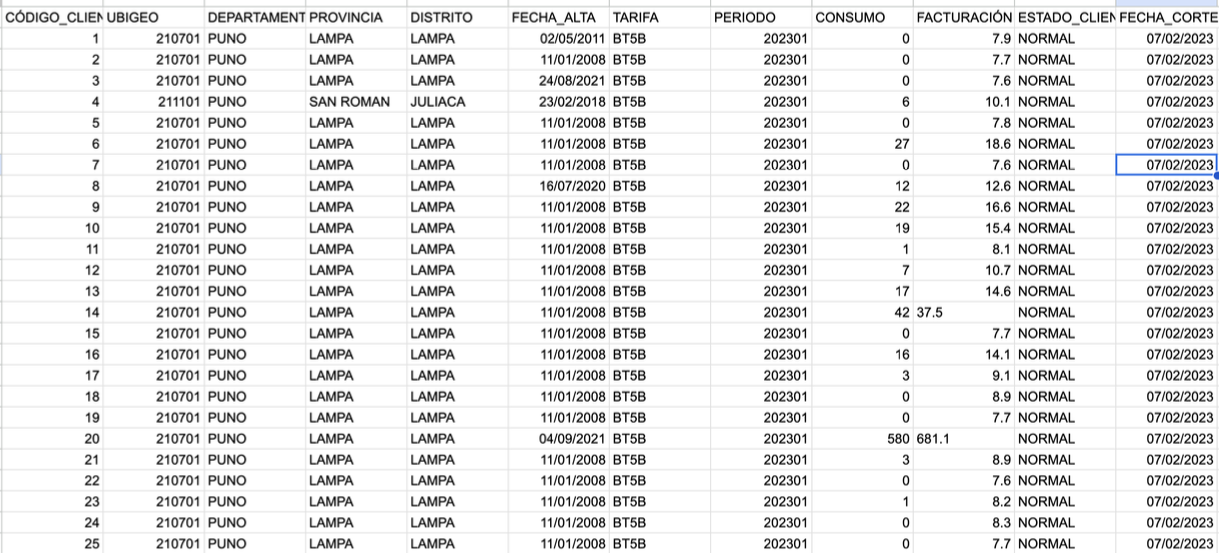
\includegraphics[width=1\textwidth]{./img/Rdatos.png}
  \caption{Muestra de datos}
  \label{Muestra de datos}
\end{figure}

\subsection{Regresion lineal simple}
La regresión lineal simple es un modelo estadístico usado para relacionar una variable independiente(X) con una variable dependiente(y). Es decir, en una regresión lineal simple solo hay dos variables (la variable explicativa X y la variable respuesta Y) y se intenta aproximar la relación que hay entre ambas variables.
\\

Nuestra variable independiente(X) es consumo
\\

Nuestra variable dependiente(y) es facturacion
\\

La ecuacion de la regresión lineal simple es:
\[
  y = \beta_0 + \beta_1x .   
\]
\begin{itemize}
  \item y = variable dependiente o variable a predecir
  \item \( \beta_0 \) = El intercepto 
  \item \( \beta_1 \) = La pendiente
\end{itemize}

El intercepto (\( \beta_0 \)) se puede calcular utilizando la ecuacion:

\[ \beta_0 = \bar{y} - \beta_1 \bar{x} \]

 La pendiente (\( \beta_1 \)) se puede calcular utilizando la fórmula:
 \[ \beta_1 = \frac{{\sum_{i=1}^{n}(x_i - \bar{x})(y_i - \bar{y})}}{{\sum_{i=1}^{n}(x_i - \bar{x})^2}} \]

\subsubsection{Usando Python}

Como estamos usando un rango de datos de 640212 para ayudarnos en el trabajo usaremos python

\begin{itemize}

  \item importamos las librerias que usaremos
\begin{lstlisting}
  import numpy as np
  import pandas as pd
  import matplotlib.pyplot as plt
  from scipy.stats import linregress
\end{lstlisting}
\item cargamos los datos y lo concatenamos
\begin{lstlisting}
  pd.options.display.float_format = '{:.2f}'.format
  enero = pd.read_csv('Enero2023.csv', encoding="ISO-8859-1", sep=";")
  febrero = pd.read_csv('febrero2023.csv', encoding="ISO-8859-1", sep=";")
  marzo = pd.read_csv('Marzo2023.csv', encoding="ISO-8859-1", sep=";")
  abril = pd.read_csv('Abril2023.csv', encoding="ISO-8859-1", sep=";")

  datos = pd.concat([enero, febrero, marzo, abril])
\end{lstlisting}
\item hacemos limpieza de datos y elegimos la variable dependiente e independiente
\begin{lstlisting}
  datos = datos.fillna(0)
  x = datos['CONSUMO']
  y = datos['FACTURACION']

\end{lstlisting}
\item la funcion linregress().shope nos permite calcular la pendiente
\item la funcion linregress.intercept nos permite calcular el intercepto
\item despues x genera un arreglo de valores en la columna consumo
\begin{lstlisting}

  #parametos de la recta
  b1 = linregress(x, y).slope #pendiente
  b0 = linregress(x, y).intercept #intercepto
  
  x = np.linspace(0, datos['CONSUMO'].max())
\end{lstlisting}
\item valor\_x es el consumo 
\item usamos la ecaucion y creamos el grafico
\item hacemos una predeccion usando la ecuacion
\begin{lstlisting}
  valor_x = 1000 
  prediccion_y = b1 * valor_x + b0
  
  datos.plot.scatter(x='CONSUMO',y='FACTURACION')
  plt.plot(x,y,'-r')
  plt.ylim(0,datos['FACTURACION'].max()*1.1)
  plt.show()
\end{lstlisting}
\end{itemize}

\subsection{Regresion Lineal Multiple}
La regresión lineal múltiple es un modelo de regresión en cual se incluyen dos o más variables independientes. Es decir, la regresión lineal múltiple es un modelo estadístico que permite relacionar varias variables explicativas con una variable respuesta de manera lineal.
\\

usaremos la siguiente ecuacion para hallar la facturacion dependiendo al consumo y el ubigeo de la persona

\[ y = \beta_0 + \beta_1x_1 + \beta_2x_2 + \ldots + \beta_nx_n \]
Son 2 variables independientes la ecuacion queda asi

\[ y = \beta_0 + \beta_1x_1 + \beta_2x_2  \]

para hallar
\[ \beta_0, \beta_1, \beta_2 \]

\[
\begin{pmatrix}
\begin{bmatrix}
  \beta_0 \\
  \beta_1 \\
  \beta_2
\end{bmatrix}
&
\begin{bmatrix}
n & \sum_{x_{1}} & \sum_{x_{2}} \\
\sum_{x_{1}} & \sum_{x_{1}^{2}} & \sum_{x_{1}x_{2}}\\
\sum_{x_{2}} & \sum_{x_{1}x_{2}} & \sum_{x_{2}^{2}} \\
\end{bmatrix}
&
\begin{bmatrix}
\sum_y \\
\sum{x_{1}y} \\ 
\sum{x_{2}y} \\ 
\end{bmatrix}
\end{pmatrix}
\]
remplazaremos la matriz

\[
\begin{pmatrix}
\begin{bmatrix}
  R1 \\
  R2 \\
  R3
\end{bmatrix}
&
\begin{bmatrix}
a  & d & c\\
d & b & d\\
c & d & c \\
\end{bmatrix}
&
\begin{bmatrix}
  1 & 0 & 0\\
  0 & 1 & 0 \\
  0 & 0 & 1 \\
\end{bmatrix}
\end{pmatrix}
\]
rempezamos convirtiendo la primera columna en 1, 0, 0
\[
\begin{pmatrix}
\begin{bmatrix}
  R1/a \\
  -d(R1)+R2 \\
  -c(R1)+R2
\end{bmatrix}
&
\begin{bmatrix}
1  & e & f\\
0 & h & i\\
0 & k & l \\
\end{bmatrix}
&
\begin{bmatrix}
  g & 0 & 0\\
  j & 1 & 0 \\
  m & 0 & 1 \\
\end{bmatrix}
\end{pmatrix}
\]
convertimos la segunda columna en 0, 1, 0
\[
\begin{pmatrix}
\begin{bmatrix}
  -e(R2)+R1 \\
  R2/h \\
  -k(R2)+R3
\end{bmatrix}
&
\begin{bmatrix}
1 & 0 & n\\
0 & 1 & x\\
0 & 1 & B \\
\end{bmatrix}
&
\begin{bmatrix}
  o & p & q\\
  y & Z & A \\
  C & D & E \\
\end{bmatrix}
\end{pmatrix}
\]
convertimos la tercera columna en 0, 0, 1
\[
\begin{pmatrix}
\begin{bmatrix}
  -h(R3)+R1 \\
  -x(R3)-R2 \\
  R3/B
\end{bmatrix}
&
\begin{bmatrix}
1 & 0 & 0\\
0 & 1 & 0\\
0 & 0 & 1 \\
\end{bmatrix}
&
\begin{bmatrix}
  F & H & I\\
  J & L & M \\
  N & O & P \\
\end{bmatrix}
\end{pmatrix}
\]
Multiplicamos las matrices
\[
\begin{pmatrix}
  \begin{bmatrix}
    F & H & I\\
    J & L & M \\
    N & O & P \\
  \end{bmatrix}
&
\begin{bmatrix}
\sum_y \\
\sum{x_{1}y} \\ 
\sum{x_{2}y} \\ 
\end{bmatrix}
\end{pmatrix}
\]
\[
\begin{pmatrix}
  \begin{bmatrix}
    \sum_y * F & \sum_y * H & \sum_y * I\\
    \sum{x_{1}y} * J & \sum{x_{1}y} * L & \sum{x_{1}y} * M \\
    \sum{x_{2}y} * N & \sum{x_{2}y} * O & \sum{x_{2}y} * P \\
  \end{bmatrix}
\end{pmatrix}
\]
resultado

\[
\begin{pmatrix}
\begin{bmatrix}
  \beta_0 \\
  \beta_1 \\
  \beta_2
\end{bmatrix}
&
\begin{bmatrix}
X \\
Y \\
Z
\end{bmatrix}
\end{pmatrix}
\]
\subsubsection {Error estandar de la estimacion multiple}
Es el error tipico cuando se emplea la ecuacion de regresion multiple para predecir la facturacion
\[
\sqrt{\frac{SCE}{{n-(k+1)}}}
\]
\begin{itemize}
  \item n = es la cantidad de la poblacion o Muestra
  \item k = es el numero de variables independientes
  \item SCE = suma de cuadrados del error o residuo
  \item para hallar SCE usamos la siguiente ecuacion
  \[
    SCE = \sum_{i}(y_i - \hat{y}_i)^2  
  \]
\end{itemize}
\subsubsection{Coeficiente de determinacion multiple }
es el porcentaje de variacion de la variable dependiente(Y) explicada por el conjunto de variables independientes(X1,X2)

\[
  R^2 = \frac{SCR}{STC}
\]
\begin{itemize}
  \item SCR = suma de cuadrados del error o residuo
  \[
    SCR = \sum_{}(\hat{y} -\bar{y} )^2  
  \] 
  \item STC = suma total de cuadrados
  \[
    STC = SCE + SCR  
  \] 
\end{itemize}
\subsubsection{Coeficiente ajustado de determinacion multiple}
El coeficiente de multiple de determinacion $R^2$ modificado para justificar el numero de variables y el tama\~no de la muestra

\[
R^2 ajustada =  1- {(1- R^2)}{\frac{n-1}{n-k-1}}
\]

Despues de hacer la metodologia y haber usado las ecuaciones usaremos python para hallar rapidamente
\\

cargamos las librerias que usaremos

\begin{lstlisting}
import numpy as np
import pandas as pd
import matplotlib.pyplot as plt
import seaborn as sns
import statsmodels.api as sm
\end{lstlisting}
importamos los datos y los concatenamos
\\ 
hacemos limpieza de datos 
\begin{lstlisting}
enero = pd.read_csv('Enero2023.csv', encoding="ISO-8859-1", sep=";")
febrero = pd.read_csv('febrero2023.csv', encoding="ISO-8859-1", sep=";")
marzo = pd.read_csv('Marzo2023.csv', encoding="ISO-8859-1", sep=";")
abril = pd.read_csv('Abril2023.csv', encoding="ISO-8859-1", sep=";")

datos = pd.concat([enero, febrero, marzo, abril])
datos = datos.fillna(0)
\end{lstlisting}
Con el metodo OLS(Ordinary Least Squares) hallamos los valores de \[ \beta_0 ,\beta_1, \beta_2 \]
 obtenemos los valores
\begin{lstlisting}
model = sm.OLS(y, X)
results = model.fit()

# Obtener los coeficientes
intercept = results.params[0]
B1 = results.params[1]
B2  = results.params[2]
\end{lstlisting}
prediciremos la facturacion con lo siguiente
\begin{lstlisting}
x1_new = 210306  # ubigeo
x2_new = 1000   # consumo

# calculamos
y= intercept + B1*x1_new + B2 * x2_new
\end{lstlisting}
Error estandar de la estimacion multiple
\begin{lstlisting}
longitudD = len(datos)
residuals = results.resid
SCE = np.sum(residuals**2)

eeem = np.sqrt(SCE/(longitudD-(2+1)))
print('Error estandar de la determinacion multiple',eeem)
\end{lstlisting}
Coeficiente de determinacion multiple

\begin{lstlisting}
promedio_facturacion = datos['FACTURACION'].mean()
y_pred = results.predict(X)

SCE = np.sum(residuals**2)
y_pred_resta_promedio = y_pred - promedio_facturacion
SCR = (y_pred_resta_promedio ** 2).sum()

STC= SCR + SCE
CDM= SCR/STC
print('Coeficiente de determinacion multiple',CDM)
\end{lstlisting}
Coeficiente ajustado de determinacion multiple

\begin{lstlisting}
coeficiente_adj_r2 = results.rsquared_adj
ccm= np.sqrt(coeficiente_adj_r2)
\end{lstlisting}

\section{Resultados}
\subsection{Regresion lineal}
Despues de hacer la metodologia y haber usado las formulas usando python podemos ver los resultados 

\begin{figure}[H]
  \centering
  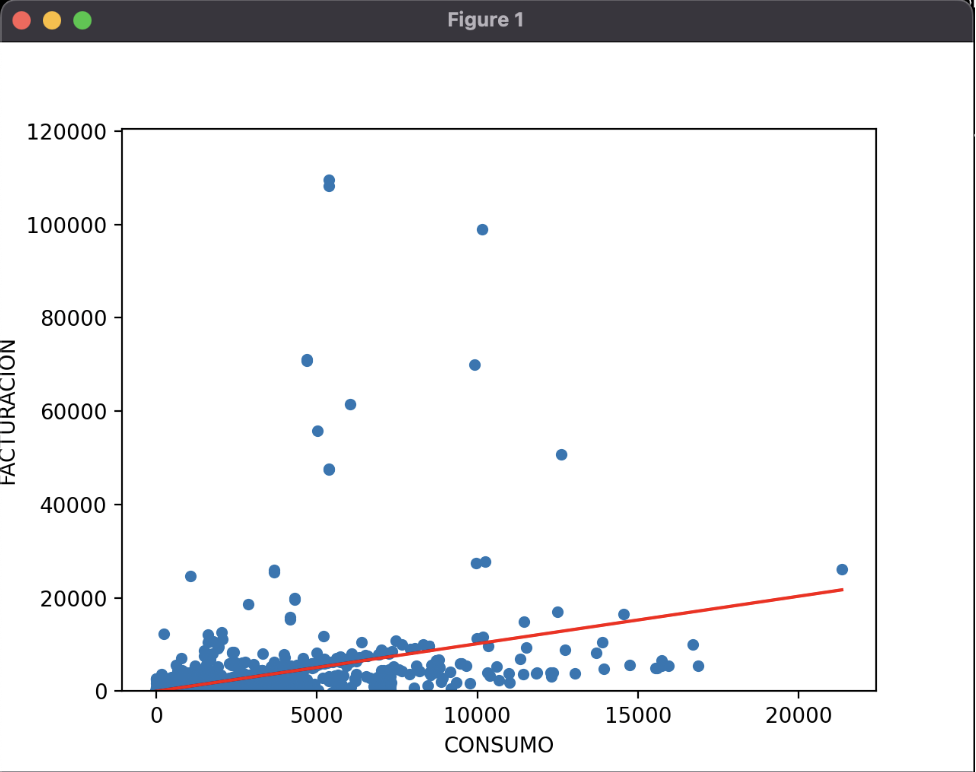
\includegraphics[width=0.8\textwidth]{./img/regrelin.png}
  \caption{Grafico de dispercion}
  \label{Grafico de dispercion}
\end{figure}
\begin{itemize}
  \item en la figura 1 se puede ver el grafico de dispercion y la linea 
\end{itemize}
usando la formula que se ejcuto en python podemos ver el resultado en este caso prediciremos la facturacion cuando el consumo sea en 1000
\\
\begin{lstlisting}
valor_x = 1000  # Valor de x para la prediccion
prediccion_y = b1 * valor_x + b0
print('Prediccion:', prediccion_y)
\end{lstlisting}
ejecutando la aplicacion valor\textunderscore x es el valor del consumo el resultado es.
\\
Predicción: 1016.309361317152
\\
Una persona que consume 1000 kwh estaria pagando 1016.30 soles
\subsection{Regresion Multiple}


en el departamento de puno provincia de carabaya distrito crucero mientras el consumo sea de 1000 llegara de facturacion 1016.27 soles

\subsubsection{Error estandar de la determinacion multiple}
el error estandar es de 314.0039251060518 de facturacion

\subsubsection{Coeficiente de determinacion multiple}
indica que el 27.60 de la variacion de la facturacion puede explicarse por el consumo y el ubigeo. En otras palabras el 72.4 se debe a otras fuentes como, como el error aleatorio o variables no incluidas en el analisis
\subsubsection{Coeficiente ajusta de determinacion multiple}
el 52.54 de la variacion de la facturacion puede explicarse por el consumo y el ubigeo. En otras palabras el 47.36 se debe a otras fuentes como, como el error aleatorio o variables no incluidas en el analisis
\subsubsection{Coeficiente de correlacion multiple}
Esta correlacion R de 0.52 es una correlacion moderada

\begin{figure}[H]
  \centering
  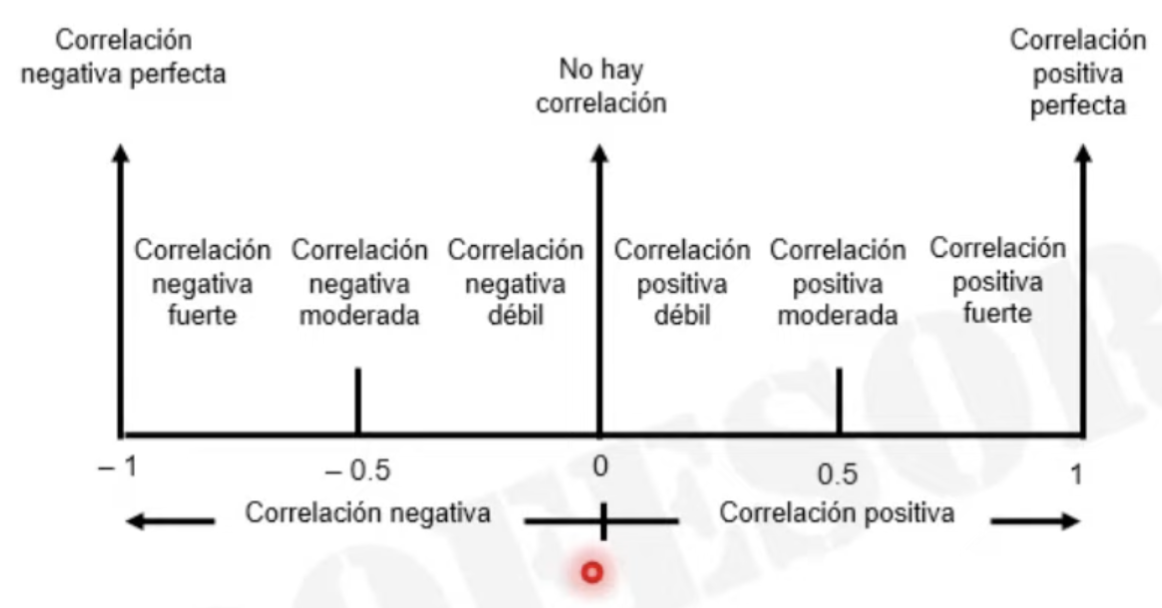
\includegraphics[width=1\textwidth]{./img/correlacion.png}
  \caption{Tabla}
  \label{Tabla}
\end{figure}
\section{Conclusiones}
Las preddicciones que nos da como resultado en regresion lineal y multiple son parecidos para que la prediccion sea mas exacta tenemos que usar mas datos en regresion multiple para tener predicciones mas exactas
\\

La regresión lineal aplicada al análisis de la facturación de la energía eléctrica en Electro Puno demostró ser una herramienta efectiva para predecir los niveles de facturación futuros.
\\

El modelo de regresión lineal desarrollado en Python mostró un buen ajuste a los datos históricos de facturación, lo que indica que puede utilizarse como una herramienta confiable para la predicción de la facturación eléctrica.
\\

Los resultados obtenidos en el estudio pueden ser utilizados por Electro Puno para planificar y gestionar de manera más eficiente la producción y distribución de energía eléctrica, optimizando los recursos y mejorando la rentabilidad.
\\

La implementación del modelo de regresión lineal en Python proporcionó una solución práctica y accesible para la predicción de la facturación eléctrica, lo que demuestra el potencial de la programación y el análisis de datos en el campo de la gestión de la energía.
\section{Referencias}


Concentracion horizontal en un ambiente regulado. El caso de la distribución de electricidad en el gran buenos aires | Revista de la Competencia y la Propiedad Intelectual. (n.d.). Retrieved June 18, 2023, from https://revistas.indecopi.gob.pe/index.php/rcpi/article/view/143 
\\

Cutipa Huarsaya, M. W. (2016). Los estados financieros y su influencia en la toma de decisiones de la Empresa Regional de Servicio Público de Electricidad - Electro Puno S. A. A. periodos 2014 - 2015. Uancv Http://Repositorio.Uancv.Edu.Pe/. https://renati.sunedu.gob.pe/handle/sunedu/2895750 
\\

Cutipa Ticona, A. C. (2016). Incidencia de la morosidad en la cartera de clientes de Electro Puno S.A.A. y su efecto en la liquidez y rentabilidad en el 2014-2015. Repositorio Institucional - UNAP. https://renati.sunedu.gob.pe/handle/sunedu/3221488
Granados , R. M. (n.d.). Modelos de regresión lineal múltiple. 
\\

Irene Moral Peláez. (n.d.).
\\

Registro Nacional de Trabajos de Investigación: Incidencia de la morosidad en la cartera de clientes de Electro Puno S.A.A. y su efecto en la liquidez y rentabilidad en el 2014-2015. (n.d.). Retrieved June 18, 2023, from https://renati.sunedu.gob.pe/handle/sunedu/3221488 
\\

Registro Nacional de Trabajos de Investigación: Los estados financieros y su influencia en la toma de decisiones de la Empresa Regional de Servicio Público de Electricidad - Electro Puno S. A. A. periodos 2014 - 2015. (n.d.). Retrieved June 18, 2023, from https://renati.sunedu.gob.pe/handle/sunedu/2895750
\end{document}
